%Este trabalho está licenciado sob a Licença Atribuição-CompartilhaIgual 4.0 Internacional Creative Commons. Para visualizar uma cópia desta licença, visite http://creativecommons.org/licenses/by-sa/4.0/deed.pt_BR ou mande uma carta para Creative Commons, PO Box 1866, Mountain View, CA 94042, USA.

\chapter{Derivadas}\label{cap_deriv}
\thispagestyle{fancy}

\section{Retas tangentes e derivadas}\label{cap_deriv_sec_retg}

Definimos a {\bf reta secante} ao gráfico de uma dada função $f$ pelos pontos $x_0$ e $x_1$, $x_0\neq x_1$, como sendo a reta determinada pela equação
\begin{equation}
  y = \frac{f(x_1)-f(x_0)}{x_1-x_0}(x-x_0)+f(x_0).
\end{equation}
Isto é, é a reta que passa pelos pontos $(x_0,f(x_0))$ e $(x_1,f(x_1))$. Veja a Figura \ref{fig:retsectg}. Observemos que o coeficiente angular da reta secante é
\begin{equation}
  m_{\text{sec}} = \frac{f(x_1)-f(x_0)}{x_1-x_0}.
\end{equation}

\begin{figure}[H]
  \centering
  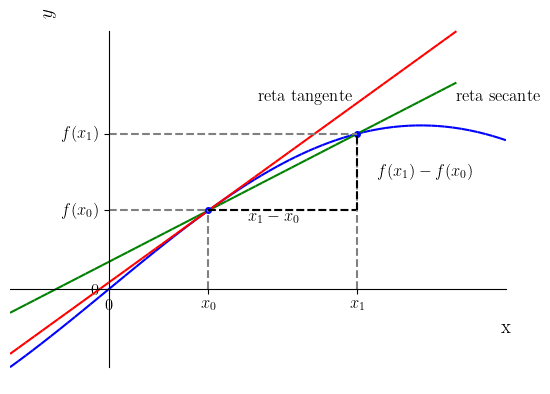
\includegraphics[width=0.7\textwidth]{./cap_deriv/dados/fig_retsectg/fig_retsectg}
  \caption{Esboços de uma reta secante (verde) e da reta tangente (vermelho) ao gráfico de uma função.}
  \label{fig:retsectg}
\end{figure}

A {\bf reta tangente} ao gráfico de uma função $f$ em $x=x_0$ é a reta que passa pelo ponto $(x_0, f(x_0))$ e tem coeficiente angular
\begin{equation}\label{eq:mtg}
  m_{\text{tg}} = \lim_{x_1\to x_0} \frac{f(x_1)-f(x_0)}{x_1-x_0}.
\end{equation}
Isto é, a reta de equação
\begin{equation}
  y = m_{\text{tg}}(x-x_0)+f(x_0).
\end{equation}
Menos formal, é a reta limite das retas secantes ao gráfico da função pelos pontos $x_0$ e $x_1$, quando $x_1\to x_0$. Veja a Figura \ref{fig:retsectg}.

\begin{obs}
  Fazendo $h = x_1-x_0$, temos que \eqref{eq:mtg} é equivalente a
  \begin{equation}
    m_{\text{tg}} = \lim_{h\to 0} \frac{f(x_0+h)-f(x_0)}{h}.
  \end{equation}
\end{obs}

\begin{ex}
  Seja $f(x)=x^2$ e $x_0 = 1$. O coeficiente angular da reta tangente ao gráfico de $f$ no ponto $x_0$ é
  \begin{align}
    m_{\text{tg}} &= \lim_{h\to 0} \frac{f(x_0+h)-f(x_0)}{h}\\
                  &= \lim_{h\to 0} \frac{(1+h)^2-1}{h}\\
                  &= \lim_{h\to 0} \frac{1+2h+h^2-1}{h}\\
                  &= \lim_{h\to 0} \frac{2+h}{1} = 2.
  \end{align}
  Assim sendo, a reta tangente ao gráfico de $f(x)=x^2$ no ponto $x_0=1$ tem coeficiente angular $m_{\text{tg}} = 2$ e equação
  \begin{equation}
    y = 2(x-1)+1 = 2x-1.
  \end{equation}
\end{ex}

\subsection{A derivada em um ponto}

A {\bf derivada} de uma função $f$ {\bf em um ponto} $x=x_0$ é denotada por $f'(x_0)$ ou $\displaystyle \frac{\dd f}{\dd x}(x_0)$ e é definida por
\begin{equation}
  f'(x_0) = \frac{\dd f}{\dd x}(x_0) = \lim_{h\to 0} \frac{f(x_0+h)-f(x_0)}{h}.
\end{equation}

\begin{ex}
  Vejamos os seguintes casos:
  \begin{enumerate}[a)]
  \item $f(x) = k$, $k$ constante.
    \begin{align}
      f'(x_0) &= \lim_{h\to 0} \frac{f(x_0+h)-f(x_0)}{h}\\
              &= \lim_{h\to 0} \frac{k-k}{h} = 0.
    \end{align}
  \item $f(x) = x$.
    \begin{align}
      f'(x_0) &= \lim_{h\to 0} \frac{f(x_0+h)-f(x_0)}{h} \\
              &= \lim_{h\to 0} \frac{x_0+h-x_0}{h} = 1.
    \end{align}
  \item $f(x) = \sqrt{x}$, $x_0=1$.
    \begin{align}
      f'(1) &= \lim_{h\to 0} \frac{\sqrt{1+h}-1}{h}\\
            &= \lim_{h\to 0} \frac{\sqrt{1+h}-1}{h}\frac{\sqrt{1+h}+1}{\sqrt{1+h}+1}\\
            &= \lim_{h\to 0} \frac{1+h-1}{h(\sqrt{1+h}+1)} = \frac{1}{2}.
    \end{align}
  \end{enumerate}
\end{ex}

\subsection*{Exercícios}

\emconstrucao

\section{Função derivada}\label{cap_deriv_sec_deriv}

\emconstrucao

\subsection*{Exercícios}

\emconstrucao
